\documentclass[USenglish,aspectratio=169]{beamer} % either 'ngerman' or 'USenglish'

\usetheme{metropolis}

\usepackage{caption}
\usepackage{subcaption}
\usepackage{babel}
\usepackage{csquotes}
\usepackage[printonlyused]{acronym}
\usepackage{xcolor}
\usepackage{colortbl}
\usepackage{hyperref}
\usepackage[
    backend=biber,
    url=false,
    style=ieee,
    citestyle=ieee
]{biblatex}
\addbibresource{bibliography.bib}

\usepackage{listings}
\usepackage{soul}

\usepackage{tabularx}
\usepackage{array}
\usepackage{multirow}
\usepackage{multicol}
\usepackage{booktabs}
\usepackage{makecell} % for line breaks in table cells

\usepackage{amsmath}
\usepackage{amsfonts}
\usepackage{amssymb}
\usepackage{amsthm}
\usepackage{centernot}
\usepackage{bm}

\usepackage{graphicx}
\usepackage{tikz}
\usepackage{pgfplots}
\usepackage{listings}

% \usepackage{appendixnumberbeamer} % might cause arithmetic overflow error!
\usepackage{glossaries}
\usepackage{adjustbox}

\usepackage{listings}
\lstset{
    basicstyle=\ttfamily\small,
    captionpos=b
    escapeinside={*@}{@*},
    showspaces=false,
    showstringspaces=false,
    showtabs=false
    xleftmargin=1pt,
    xrightmargin=1pt,
    aboveskip=1pt,
    belowskip=1pt,
    columns=fullflexible
}
\setlength\fboxsep{1pt}

\title{Expressing \acsp{CRDT} with Datalog}
\subtitle{Master's Thesis in Data Engineering and Analytics}
\author{
    \textbf{Leo Stewen} \\ \\
    Examiner: Prof. Dr. Viktor Leis \\
    Supervisor: Dr. Martin Kleppmann \\
}
\date{5th August 2025}
\institute[TUM]{\textbf{Technical University of Munich}}

\graphicspath{{figures/}{../figures/}}
\hypersetup{
    pdftitle=\title,
    pdfauthor=\author,
    bookmarksopen=true,
    hidelinks,
}

\metroset{numbering=fraction,progressbar=frametitle,block=fill}
\setbeamertemplate{section in toc}[sections numbered]
% \setbeamercovered{transparent=35}
\setbeamercovered{invisible}

\usetikzlibrary{
    quotes,
    automata,
    positioning,
    arrows,
    arrows.meta,
    calc,
    backgrounds,
    decorations.pathreplacing,
    calc,
    positioning,
    fit
}

\definecolor{TUMBlue}{HTML}{0065BD}
\definecolor{TUMSecondaryBlue}{HTML}{005293}
\definecolor{TUMSecondaryBlue2}{HTML}{003359}
\definecolor{TUMBlack}{HTML}{000000}
\definecolor{TUMWhite}{HTML}{FFFFFF}
\definecolor{TUMDarkGray}{HTML}{333333}
\definecolor{TUMGray}{HTML}{808080}
\definecolor{TUMLightGray}{HTML}{CCCCC6}
\definecolor{TUMAccentGray}{HTML}{DAD7CB}
\definecolor{TUMAccentOrange}{HTML}{E37222}
\definecolor{TUMAccentGreen}{HTML}{A2AD00}
\definecolor{TUMAccentLightBlue}{HTML}{98C6EA}
\definecolor{TUMAccentBlue}{HTML}{64A0C8}

\newcommand{\setop}[5][set]{$\mathit{#1}_{#2}^{#3} (#4, #5)$}
\tikzset{
    op/.style={
        font=\footnotesize,
        state,
        minimum size=56.0pt,
        fill=white,
        scale=0.9,
    },
    head/.style={
        op,
        accepting,
    },
    edge/.style={
        ->,
        >={Stealth[round]},
    },
    pred/.style={
        edge,
    },
}

\newcommand{\backupbegin}{
   \newcounter{framenumberappendix}
   \setcounter{framenumberappendix}{\value{framenumber}}
}
\newcommand{\backupend}{
   \addtocounter{framenumberappendix}{-\value{framenumber}}
   \addtocounter{framenumber}{\value{framenumberappendix}}
}

\begin{document}

\begin{frame}
    \maketitle
\end{frame}

\setbeamercovered{transparent=50}
\begin{frame}
    \begin{itemize}
        \visible<1->{\onslide<1-2>{
        \item[ ] \textbf{Idea: Define \acsp{CRDT} in Datalog}
        }}
        \visible<2->{\onslide<2>{
        \item[\(\Rightarrow\)] declarative, concise language to work with
        }}
        \visible<3->{\onslide<3-4>{
        \item[+] Deterministic execution on top of a
                 \emph{monotonically growing set} of operations
        }}
        \visible<4->{\onslide<4>{
        \item[\(\Rightarrow\)] guaranteed convergence (!)
        }}
        \visible<5->{\onslide<5-6>{
        \item[+] Query engine based on \acl{IVM}
        }}
        \visible<6->{\onslide<6>{
        \item[\(\Rightarrow\)] competitive performance (?)
        }}
    \end{itemize}
\end{frame}
\setbeamercovered{invisible}

\begin{frame}[standout]
    \begin{center}
        Excursion
    \end{center}
\end{frame}

\begin{frame}{What are \acsp{CRDT}?}
    \onslide<1->{
    \Acfp{CRDT} are a class of data structures that allow replicas in a distributed
    system to converge to a consistent shared state without any coordination
    of reads and writes to the data structure.
    }

    \onslide<2->{
    \(\Rightarrow\) concurrent writes which exhibit no order are inevitable
    }
\end{frame}

\begin{frame}{\acsp{CRDT} for Database People}
    \begin{center}
        \textit{``\acsp{CRDT} are similar to \acs{OCC} but without the aborts''}
    \end{center}

    \pause
    \begin{table}
        \center
        \begin{tabular}{@{} l l l @{}}
            \toprule
                                & \acs{OCC}                       & \acs{CRDT}                    \\
            \midrule
            Use Case             & Synchronization of shared data & Replication of shared data    \\
            \pause
            Objects              & Transactions                   & Operations                    \\
            \pause
            Actors               & Threads                        & Replicas                      \\
            \pause
            Time                 & Wall-clock time                & Causal Time                   \\
            \pause
            Concurrency Behavior & \emph{Abort}                   & \emph{Merge and Converge}     \\
            \bottomrule
        \end{tabular}
    \end{table}

    % Upon concurrent writes, \acs{OCC} aborts some transaction(s),
    % while \acsp{CRDT} merge operations to
    % \emph{converge to the same state across replicas}.
\end{frame}

\begin{frame}[fragile]{Why not SQL?}
    \begin{figure}[h]
        \centering
        \begin{lstlisting}[keepspaces]
            WITH RECURSIVE ??? AS (
                SELECT from, to, weight, 1 AS hopcnt
                FROM edge
                WHERE from = 2
                UNION ALL
                SELECT c.from, e.to, c.weight + e.weight, c.hopcnt + 1
                FROM closure c
                JOIN edge e ON c.to = e.from
            )

            SELECT * FROM ???;\end{lstlisting}
        \caption{Transitive closure with SQL.}
    \end{figure}
\end{frame}

\begin{frame}[fragile]{Isn't Datalog dead (yet)?}
    \begin{figure}[h]
        \centering
        % edge(from, to, weight)       :- .
        \begin{lstlisting}[keepspaces]
closure(from, to, weight, 1) :- edge(from, to, weight), from = 2.

closure(from, to, cweight + weight, hopcnt + 1)
                             :- closure(from, via, cweight, hopcnt),
                                edge(via, to, weight).\end{lstlisting}
        \caption{Transitive closure with Datalog.}\label{code:trans-closure-datalog}
    \end{figure}
\end{frame}

\setbeamercovered{transparent=50}
\begin{frame}
    \begin{itemize}
        \visible<1->{\onslide<1-2>{
        \item[ ] \textbf{Idea: Define \acsp{CRDT} in Datalog}
        }}
        \visible<1->{\onslide<1>{
        \item[\(\Rightarrow\)] declarative, concise language to work with
        \item[+] Deterministic execution on top of a
                 \emph{monotonically growing set} of operations
        \item[\(\Rightarrow\)] guaranteed convergence (!)
        \item[+] Query engine based on \acl{IVM}
        \item[\(\Rightarrow\)] competitive performance (?)
        }}
    \end{itemize}
\end{frame}
\setbeamercovered{invisible}

\begin{frame}{Example: Key-value store \acs{CRDT} with \aclp{MVR}}
    \begin{columns}
        \begin{column}{0.4\textwidth}
            \begin{figure}
                \centering
                \begin{tabular}{@{}llll@{}}
                    \toprule
                    RepId   & Ctr    & Key     & Value   \\
                    \midrule
                    \(r_1\) & 1      & \(k_1\) & \(v_1\) \\
                    \(r_1\) & 2      & \(k_1\) & \(v_2\) \\
                    \(r_2\) & 2      & \(k_1\) & \(v_3\) \\
                    \midrule
                    \ldots  & \ldots & \ldots  & \ldots  \\
                    \midrule
                    \(r_1\) & 3      & \(k_2\) & \(u_1\) \\
                    \(r_2\) & 4      & \(k_2\) & \(u_2\) \\
                    \(r_2\) & 5      & \(k_2\) & \(u_3\) \\
                    \bottomrule
                \end{tabular}
                \caption{Set Relation}
            \end{figure}
        \end{column}
        \begin{column}{0.6\textwidth}
            \begin{figure}
                \centering
                \begin{tabular}{@{}llll@{}}
                    \toprule
                    FromRepId & FromCtr & ToRepId & ToCtr  \\
                    \midrule
                    \(r_1\)   & 1       & \(r_1\) & 2      \\
                    \(r_1\)   & 1       & \(r_2\) & 2      \\
                    \midrule
                    \ldots    & \ldots  & \ldots  & \ldots \\
                    \midrule
                    \(r_1\)   & 3       & \(r_2\) & 5      \\
                    \(r_2\)   & 4       & \(r_2\) & 5      \\
                    \bottomrule
                \end{tabular}
                \caption{Pred Relation}
            \end{figure}
        \end{column}
    \end{columns}
\end{frame}

\begin{frame}{Example: Key-value store \acs{CRDT} with \aclp{MVR}}
    \small
    \def\dist{15pt}
    \begin{columns}
        \begin{column}{0.5\textwidth}
            \begin{figure}
                \centering
                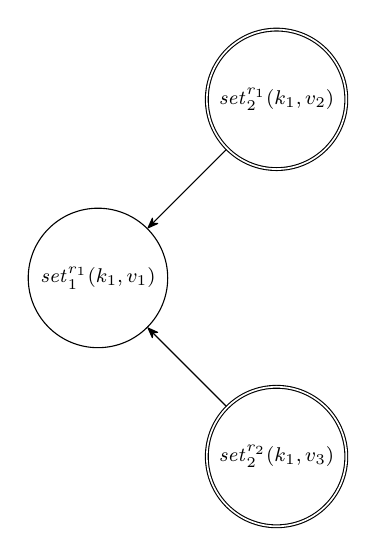
\begin{tikzpicture}
                    % nodes and edges
                    \node[op] (k10) {\setop{1}{r_1}{k_1}{v_1}};
                    \node[head,above right=\dist of k10] (k11) {\setop{2}{r_1}{k_1}{v_2}} edge [pred] (k10);
                    \node[head,below right=\dist of k10] (k12) {\setop{2}{r_2}{k_1}{v_3}} edge [pred] (k10);
                \end{tikzpicture}
                \caption{Causal history of register \(k_1\)}\label{fig:causal-history-k1}
            \end{figure}
        \end{column}
        \begin{column}{0.5\textwidth}
            \begin{figure}
                \centering
                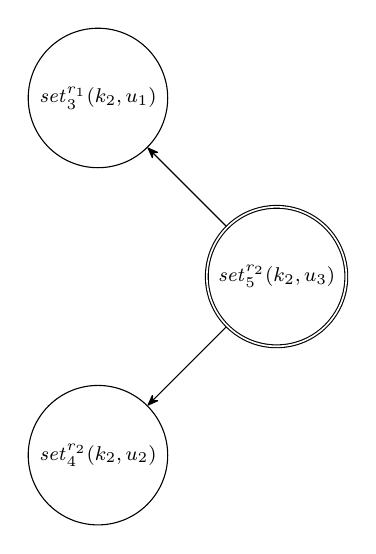
\begin{tikzpicture}
                    % nodes and edges
                    \node[op] (k20) {\setop{3}{r_1}{k_2}{u_1}};
                    \node[head,below right=\dist of k20] (k22) {\setop{5}{r_2}{k_2}{u_3}} edge [pred] (k20);
                    \node[op,below left=\dist of k22] (k21) {\setop{4}{r_2}{k_2}{u_2}};
                    \draw [pred] (k22) edge (k21);
                \end{tikzpicture}
                \caption{Causal history of register \(k_2\)}\label{fig:causal-history-k2}
            \end{figure}
        \end{column}
    \end{columns}
\end{frame}

\begin{frame}[fragile]{Example: Key-value store \acs{CRDT} with \aclp{MVR}}
    \begin{figure}
        \centering
        \begin{lstlisting}[keepspaces]
overwritten(RepId, Ctr) :- pred(RepId, Ctr, _, _).
mvrStore(Key, Value)    :- set(RepId, Ctr, Key, Value),
                           not overwritten(RepId, Ctr).\end{lstlisting}
        \caption{Datalog query for the key-value store.}\label{code:mvr-store-datalog}
    \end{figure}

    Result: \(\{ (k_1, v_2), (k_1, v_3), (k_2, u_3) \}\)
\end{frame}

\setbeamercovered{transparent=50}
\begin{frame}
    \begin{itemize}
        \visible<1->{\onslide<1>{
        \item[ ] \textbf{Idea: Define \acsp{CRDT} in Datalog}
        \item[\(\Rightarrow\)] declarative, concise language to work with
        }}
        \visible<2->{\onslide<2>{
        \item[+] Deterministic execution on top of a
                 \emph{monotonically growing set} of operations
        }}
        \invisible<0->{
        \item[\(\Rightarrow\)] guaranteed convergence (!)
        \item[+] Query engine based on \acl{IVM}
        \item[\(\Rightarrow\)] competitive performance (?)
        }
    \end{itemize}
\end{frame}
\setbeamercovered{invisible}

\begin{frame}{Why is proving the correctness of \acsp{CRDT} so hard?}
    It has to be proven that replicas with the same set of updates
    converge to the same state \emph{under all possible concurrent executions}.

    \pause
    Currently, application developers have to choose between:
    \begin{itemize}
        \item implement and prove a custom \ac{CRDT} from scratch
              (very hard~\cite{kleppmann2022assessing,gomes2017verifying})
        \item use an off-the-shelf \ac{CRDT} library like Automerge~\cite{automerge}
              (inflexible)
        \item learn a \acs{DSL} which guarantees convergence~\cite{verifx,lore,propel}
    \end{itemize}
\end{frame}

\begin{frame}{Guaranteed Convergence}
    We define a state-based \acsp{CRDT} whose state \(S\) is the set
    of operations to the \ac{CRDT}.

    Merge function: \( S_1 \cup S_2 \)
    \begin{itemize}
        \item[\checkmark] \textbf{Idempotent}
                          % \( S_1 \cup S_1 = S_1 \)
        \item[\checkmark] \textbf{Commutative}
                          % \( S_1 \cup S_2 = S_2 \cup S_1 \)
        \item[\checkmark] \textbf{Associative}
                          % \( (S_1 \cup S_2) \cup S_3 = S_1 \cup (S_2 \cup S_3) \)
    \end{itemize}

    Applying any \emph{pure} function \(f: S \to T\) preserves the convergence property.
\end{frame}

\setbeamercovered{transparent=50}
\begin{frame}
    \begin{itemize}
        \visible<0->{\onslide<0>{
        \item[ ] \textbf{Idea: Define \acsp{CRDT} in Datalog}
        \item[\(\Rightarrow\)] declarative, concise language to work with
        }}
        \visible<1->{\onslide<1>{
        \item[+] Deterministic execution on top of a
                 \emph{monotonically growing set} of operations
        \item[\(\Rightarrow\)] guaranteed convergence (!)
        }}
        \visible<2->{\onslide<2>{
        \item[+] Query engine based on \acl{IVM}
        }}
        \invisible<1->{
        \item[\(\Rightarrow\)] competitive performance (?)
        }
    \end{itemize}
\end{frame}
\setbeamercovered{invisible}

\begin{frame}{Access Patterns with \acsp{CRDT}}
    \begin{itemize}
        \item \textbf{Hydration} (application startup).
        \item \textbf{Near-real-time} (application runtime).
        \item[\(\Rightarrow\)] \acf{IVM} based on DBSP~\cite{budiu2025dbsp,budiu2024dbsp}.
    \end{itemize}
\end{frame}

\begin{frame}[fragile]{Incremental Query Engine}
    \begin{figure}
        \centering
        \begin{tabular}{c}
            \begin{lstlisting}[keepspaces]
mvrStore(Key, Value) :- set(RepId, Ctr, Key, Value),
                        isCausallyReady(RepId, Ctr),
                        not overwritten(RepId, Ctr).\end{lstlisting}
        \end{tabular}
        \caption{The ``mvrStore'' rule with the ``isLeaf'' predicate inlined.}\label{code:mvr-store-rule-inlined}
    \end{figure}

    \vspace{1em}

    \begin{figure}
        \centering
        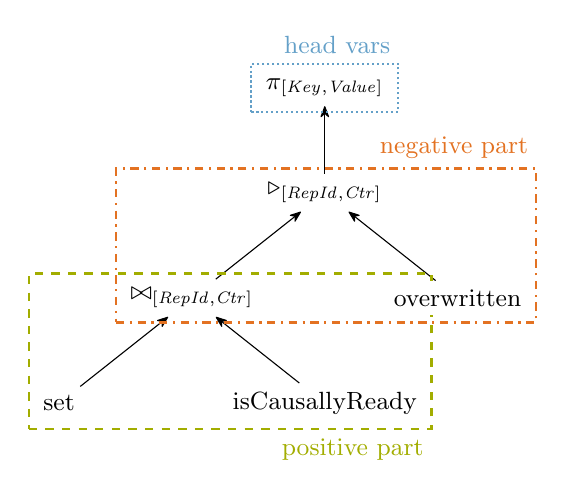
\begin{tikzpicture}
            \small

            \tikzset{
                node distance=38pt and 48pt,
                on grid,
                node/.style={rectangle,minimum width=0pt,minimum height=0pt,align=center,fill=white},
                input/.style={edge},
                edgelabel/.style={midway},
                pipeline/.style={rectangle,thick,draw=gray,inner sep=2pt},
            }

            \node[node] (projection) {\(\pi_{[\mathit{Key}, \mathit{Value}]}\)};
            \node[node,below=of projection] (antijoin) {\(\triangleright_{[\mathit{RepId}, \mathit{Ctr}]}\)};

            \node[node,below left=of antijoin] (equijoin) {\(\bowtie_{[\mathit{RepId}, \mathit{Ctr}]}\)};
            \node[node,below right=of antijoin] (overwritten) {overwritten};

            \node[node,below left=of equijoin] (set) {set};
            \node[node,below right=of equijoin] (caus) {isCausallyReady};

            \begin{scope}[on background layer]
                \draw[input] (antijoin) to[] (projection);

                \draw[input] (overwritten) to[] (antijoin);
                \draw[input] (equijoin) to[] (antijoin);

                \draw[input] (set) to[] (equijoin);
                \draw[input] (caus) to[] (equijoin);

                \node[pipeline,draw=TUMAccentGreen,dashed,fit=(set) (caus) (equijoin)] (pospart) {};
                \node[anchor=north east,color=TUMAccentGreen] at (pospart.south east) {positive part};

                \node[pipeline,draw=TUMAccentOrange,dashdotted,fit=(equijoin) (antijoin) (overwritten)] (negpart) {};
                \node[anchor=south east,color=TUMAccentOrange] at (negpart.north east) {negative part};

                \node[pipeline,draw=TUMAccentBlue,densely dotted,fit=(projection)] (headpart) {};
                \node[anchor=south east,color=TUMAccentBlue] at (headpart.north east) {head vars};
            \end{scope}
        \end{tikzpicture}
        \caption{Query plan with an antijoin to handle the negative ``overwritten'' atom.}\label{fig:negative-query-plan}
    \end{figure}
\end{frame}

\setbeamercovered{transparent=50}
\begin{frame}
    \begin{itemize}
        \visible<0->{\onslide<0>{
        \item[ ] \textbf{Idea: Define \acsp{CRDT} in Datalog}
        \item[\(\Rightarrow\)] declarative, concise language to work with
        \item[+] Deterministic execution on top of a
                 \emph{monotonically growing set} of operations
        \item[\(\Rightarrow\)] guaranteed convergence (!)
        }}
        \visible<1->{\onslide<1>{
        \item[+] Query engine based on \acl{IVM}
        \item[\(\Rightarrow\)] competitive performance (?)
        }}
    \end{itemize}
\end{frame}
\setbeamercovered{invisible}

\begin{frame}{Competitive Performance}
\end{frame}

\setbeamercovered{transparent=50}
\begin{frame}{What we don't know yet}
    \begin{itemize}
        \visible<1->{\onslide<1>{
        \item \textbf{Expressiveness}: Are there \acsp{CRDT} that cannot be
              expressed in Datalog?
        }}
        \visible<2->{\onslide<2>{
        \item \textbf{Performance}: How does the performance compare to existing
              (both verified and unverified) \acsp{CRDT} libraries?
              To other \acs{DSL}-based approaches?
        }}
    \end{itemize}

    \visible<3->{\onslide<3>{
    \begin{center}
        \textit{What is the price to pay for guaranteed convergence?}
    \end{center}
    }}
\end{frame}

\begin{frame}[standout]
    \begin{center}
        Questions?
    \end{center}
\end{frame}

\begin{frame}{Abbreviations}
\begin{acronym}
    \itemsep-.25\baselineskip
    \acro{TUM}[TUM]{Technical University of Munich}
    \acro{OCC}[OCC]{optimistic concurrency control}
    \acro{CRDT}[CRDT]{convergent replicated data type}
    \acro{IR}[IR]{intermediate representation}
    \acro{AST}[AST]{abstract syntax tree}
    \acro{EDBP}[EDBP]{extensional database predicate}
    \acro{IDBP}[IDBP]{intensional database predicate}
    \acro{MVR}[MVR]{multi-valued register}
    \acro{LWWR}[LWWR]{last-writer-wins register}
    \acro{IVM}[IVM]{incremental view maintenance}
    \acro{GUI}[GUI]{graphical user interface}
    \acro{API}[API]{application programming interface}
    \acro{SAT}[SAT]{satisfiability}
    \acro{DSL}[DSL]{domain-specific language}
    \acro{RGA}[RGA]{replicated growable arrays}
\end{acronym}
\end{frame}

\begin{frame}[allowframebreaks]{References}
    \printbibliography[heading=none]
\end{frame}

% TODO: Appendix with List CRDT

\appendix

\backupbegin

\begin{frame}{Key-value store \acs{CRDT} with \acsp{MVR} and causal broadcast}
\end{frame}

\begin{frame}{List CRDT}
\end{frame}

\backupend

\end{document}
